\begin{exampleblock}{Background}
%TODO Change text about utility and risk sensitivites to a comic
%TODO Change text color of captions
%TODO Include information about exp UF and include the formula

\Large{Risk and Utility}

\normalsize

\begin{itemize}
    \item Risk is induced by choice with uncertain outcome.
    \item People behave \textbf{risk seeking}, \textbf{risk neutral} or \textbf{risk averse}.
    % \item Risk can exist without the danger of loss (e.g. loosing money).
    \item People map money to utility by \textbf{utility functions}, e.g. exponential utility $U(a) = (1-\exp(-\lambda a)) / \lambda$. 
    %\item The same amount of money can have different utility for different people.
    \item Curvature of function defines risk profile.
\end{itemize}

\hspace{2cm}


\newlength{\twosubht}
\newsavebox{\twosubbox}


\begin{figure}[htp]

% preliminary
\sbox\twosubbox{%
  \resizebox{\dimexpr.9\textwidth-1em}{!}{%
    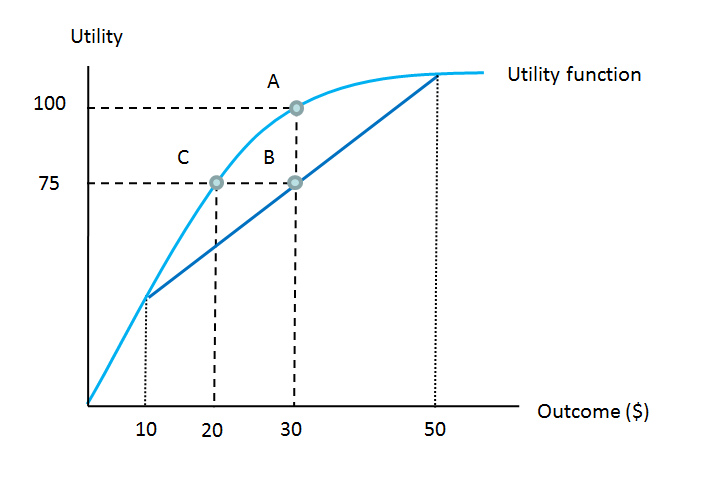
\includegraphics[height=10cm]{img/background/riskaversion}%
    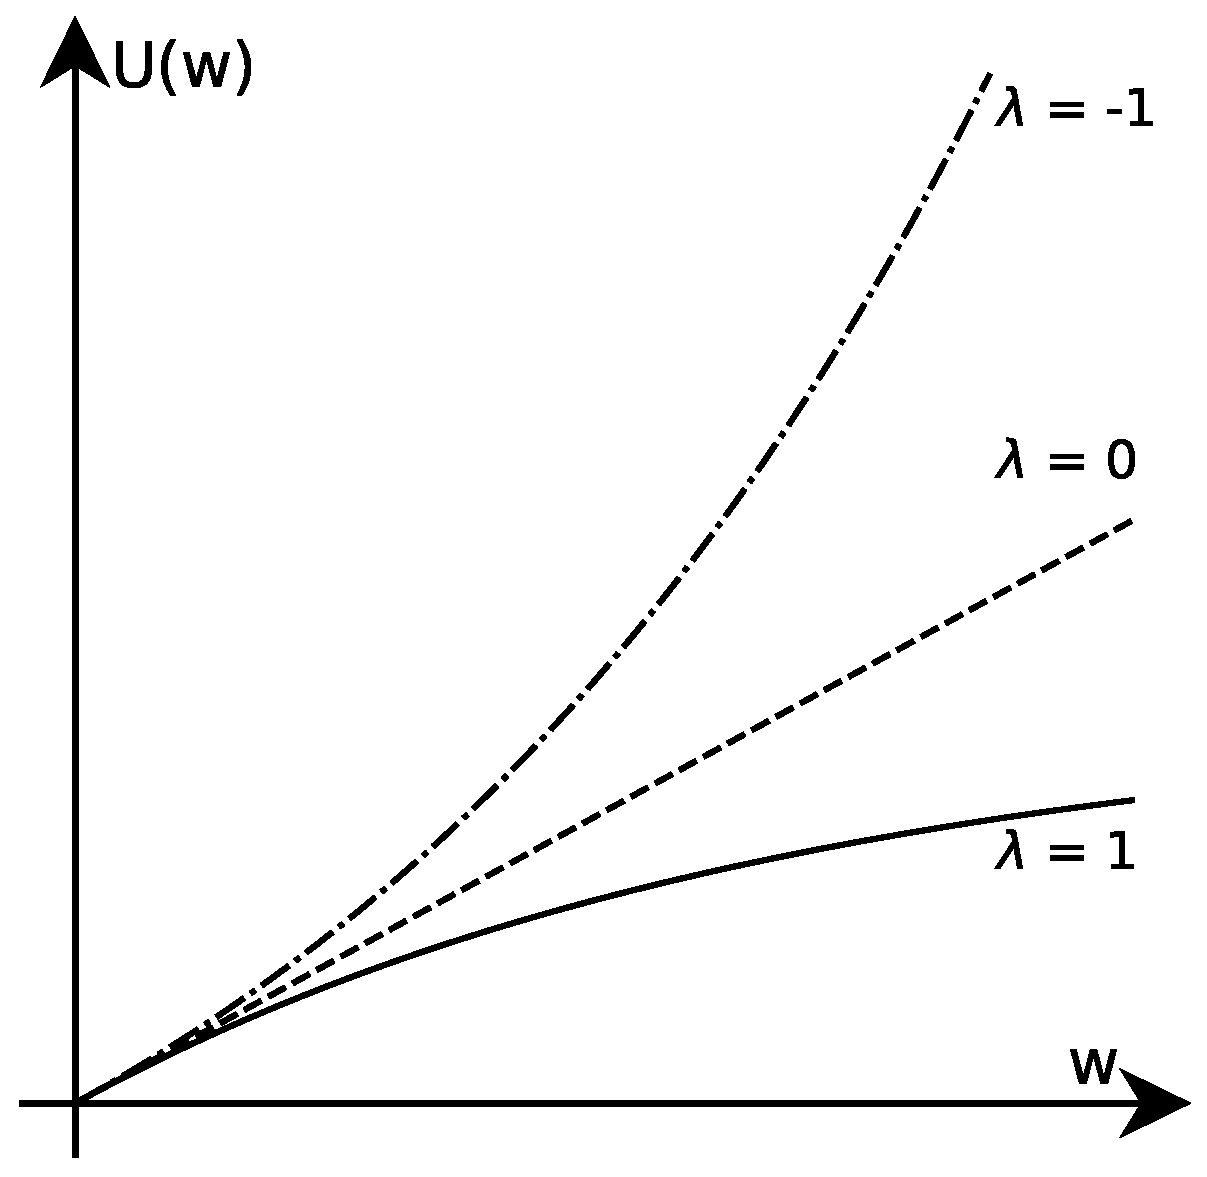
\includegraphics[height=10cm]{img/background/Exponential_Utility_Function}%
  }%
}
\setlength{\twosubht}{\ht\twosubbox}

% typeset

\centering

\subcaptionbox{Risk averse lottery\label{f}}{%
  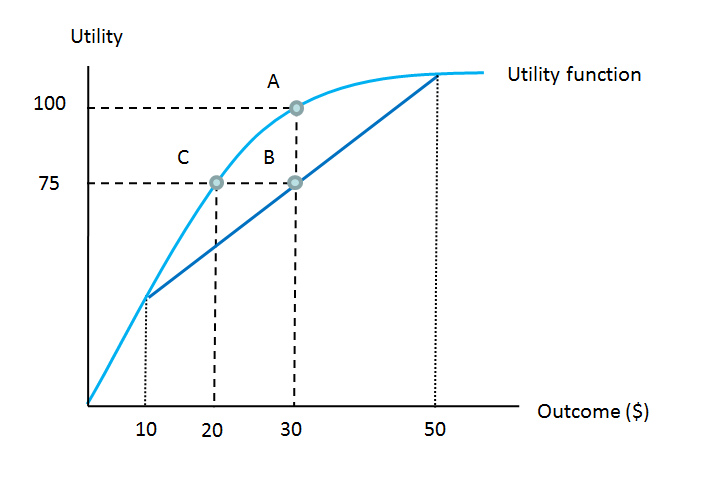
\includegraphics[height=\twosubht]{img/background/riskaversion}%
}\quad
\subcaptionbox{Exponential utility function\label{s}}{%
  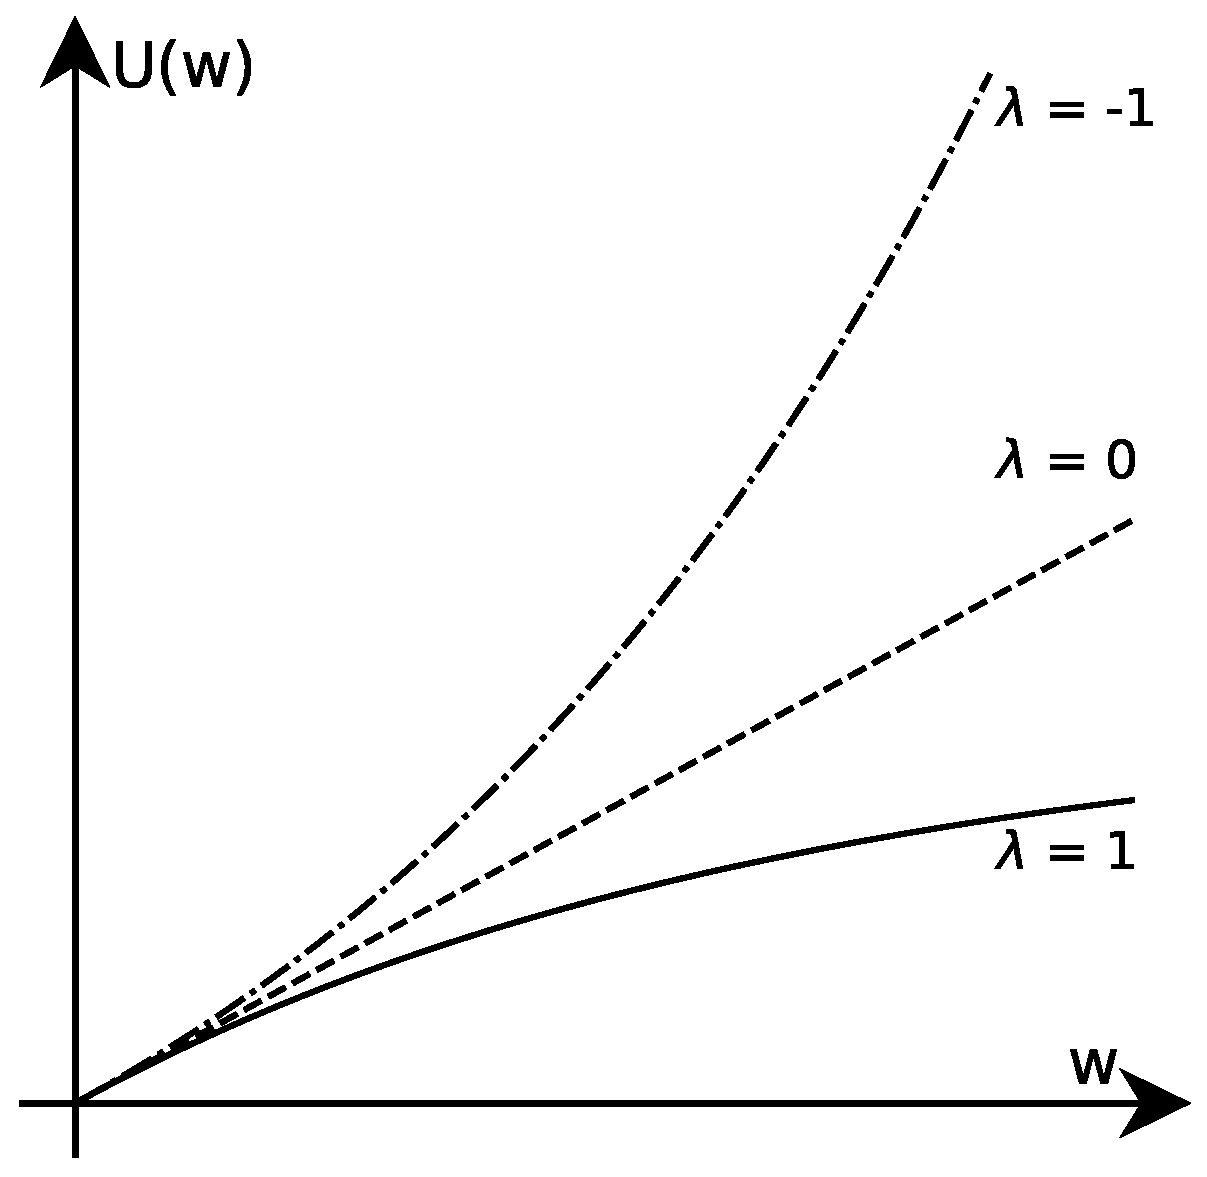
\includegraphics[height=\twosubht]{img/background/Exponential_Utility_Function}%
}

\caption{a) Choice from a risk free gift of 30\$ or a lottery where by coin flip you win 10\$ or 50\$. The utility for the risk free choice (point A) is higher than the expected utility of the risky lottery (point B). b) The exponential utility function for different risk parameters $\alpha$. $a < 0$ implies risk seeking, $a = 0 $ risk neutral and $a > 0 $ risk averse behaviour.}

\end{figure}


\Large{(Partially Observable) Markov Decision Process}

\normalsize
\begin{itemize}
    \item Making decisions when state is not fully-observable.
    \item Work on probability distribution over states rather than actual state.
\end{itemize}

\hspace{2cm}


\begin{figure}
  \centering
    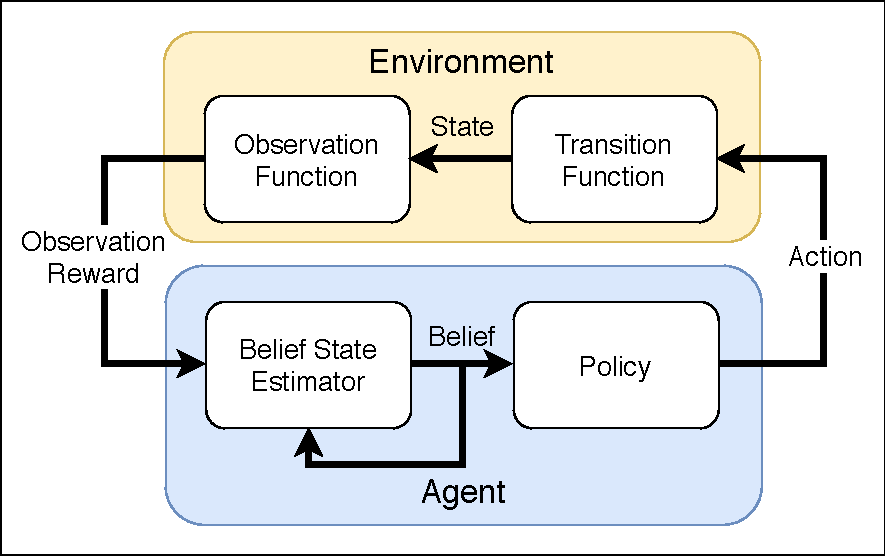
\includegraphics[width=0.7\textwidth]{img/background/POMDP}
  \caption{Sketch of a partially observable environment. The agent only gets observations as inputs.}
\end{figure}


%\begin{itemize}
%    \item Set of States $\mathcal{S}$ (Terminal and Non Terminal)
%    \item Set of Actions $\mathcal{A}$
%    \item Probabilistic Transitions depending on tuple $\mathcal{S} x \mathcal{A}$
%    \item Reward function $R(s,a)$
%\end{itemize}

%For partially observability states are hidden but produce observations:
%\begin{itemize}
%    \item Observation space $\mathcal{O}$
%    \item Observation function $p(o | s, a)$
%\end{itemize}

% add reference: http://www.cassandra.org/arc/papers/aaai94.pdf


\end{exampleblock}
